\chapter{Extensibilidad}\label{chapter:extensibility}
Uno de los objetivos de este trabajo es la creación de una herramienta que 
permita la posterior integración de procesos de administración y planificación 
que se llevan a cabo en la Facultad de Matemática y Computación de la Universidad
de La Habana. 
En este capítulo propone una guía de cómo agregar nuevos 
procesos al sistema de gestión que se implementó.

En la siguiente sección se describe cómo están estructurados los proyectos 
servidor y cliente. 

\section{Estructura del cliente y servidor}
El desarrollo en el lado del servidor se llevó a cabo con el  
uso de la biblioteca Django, en particular Django Rest Framework.
Para el desarrollo de los procesos de asignación de docencia y planificaciones de las 
tesis se crearon dos apps independientes de Django, con el objetivo de agrupar los ficheros 
necesarios para la modelación de cada proceso. 
En la figura \ref{img-server-structure} se muestra cómo está estructurado el servidor.




% Para la creación del proyecto se utilizó el siguiente comando.


% \begin{verbatim}
%     django-admin startproject <nombre_del_proyecto>
% \end{verbatim}

%  Para la creación de las apps de Django se 
% utilizó el comando siguiente.

% \begin{verbatim}
%     python manage.py startapp <nombre_de_la_app>
% \end{verbatim}

% Como resultado se obtuvo la siguiente estructura que se muestra 
% en la figura .

\begin{figure}[H]
    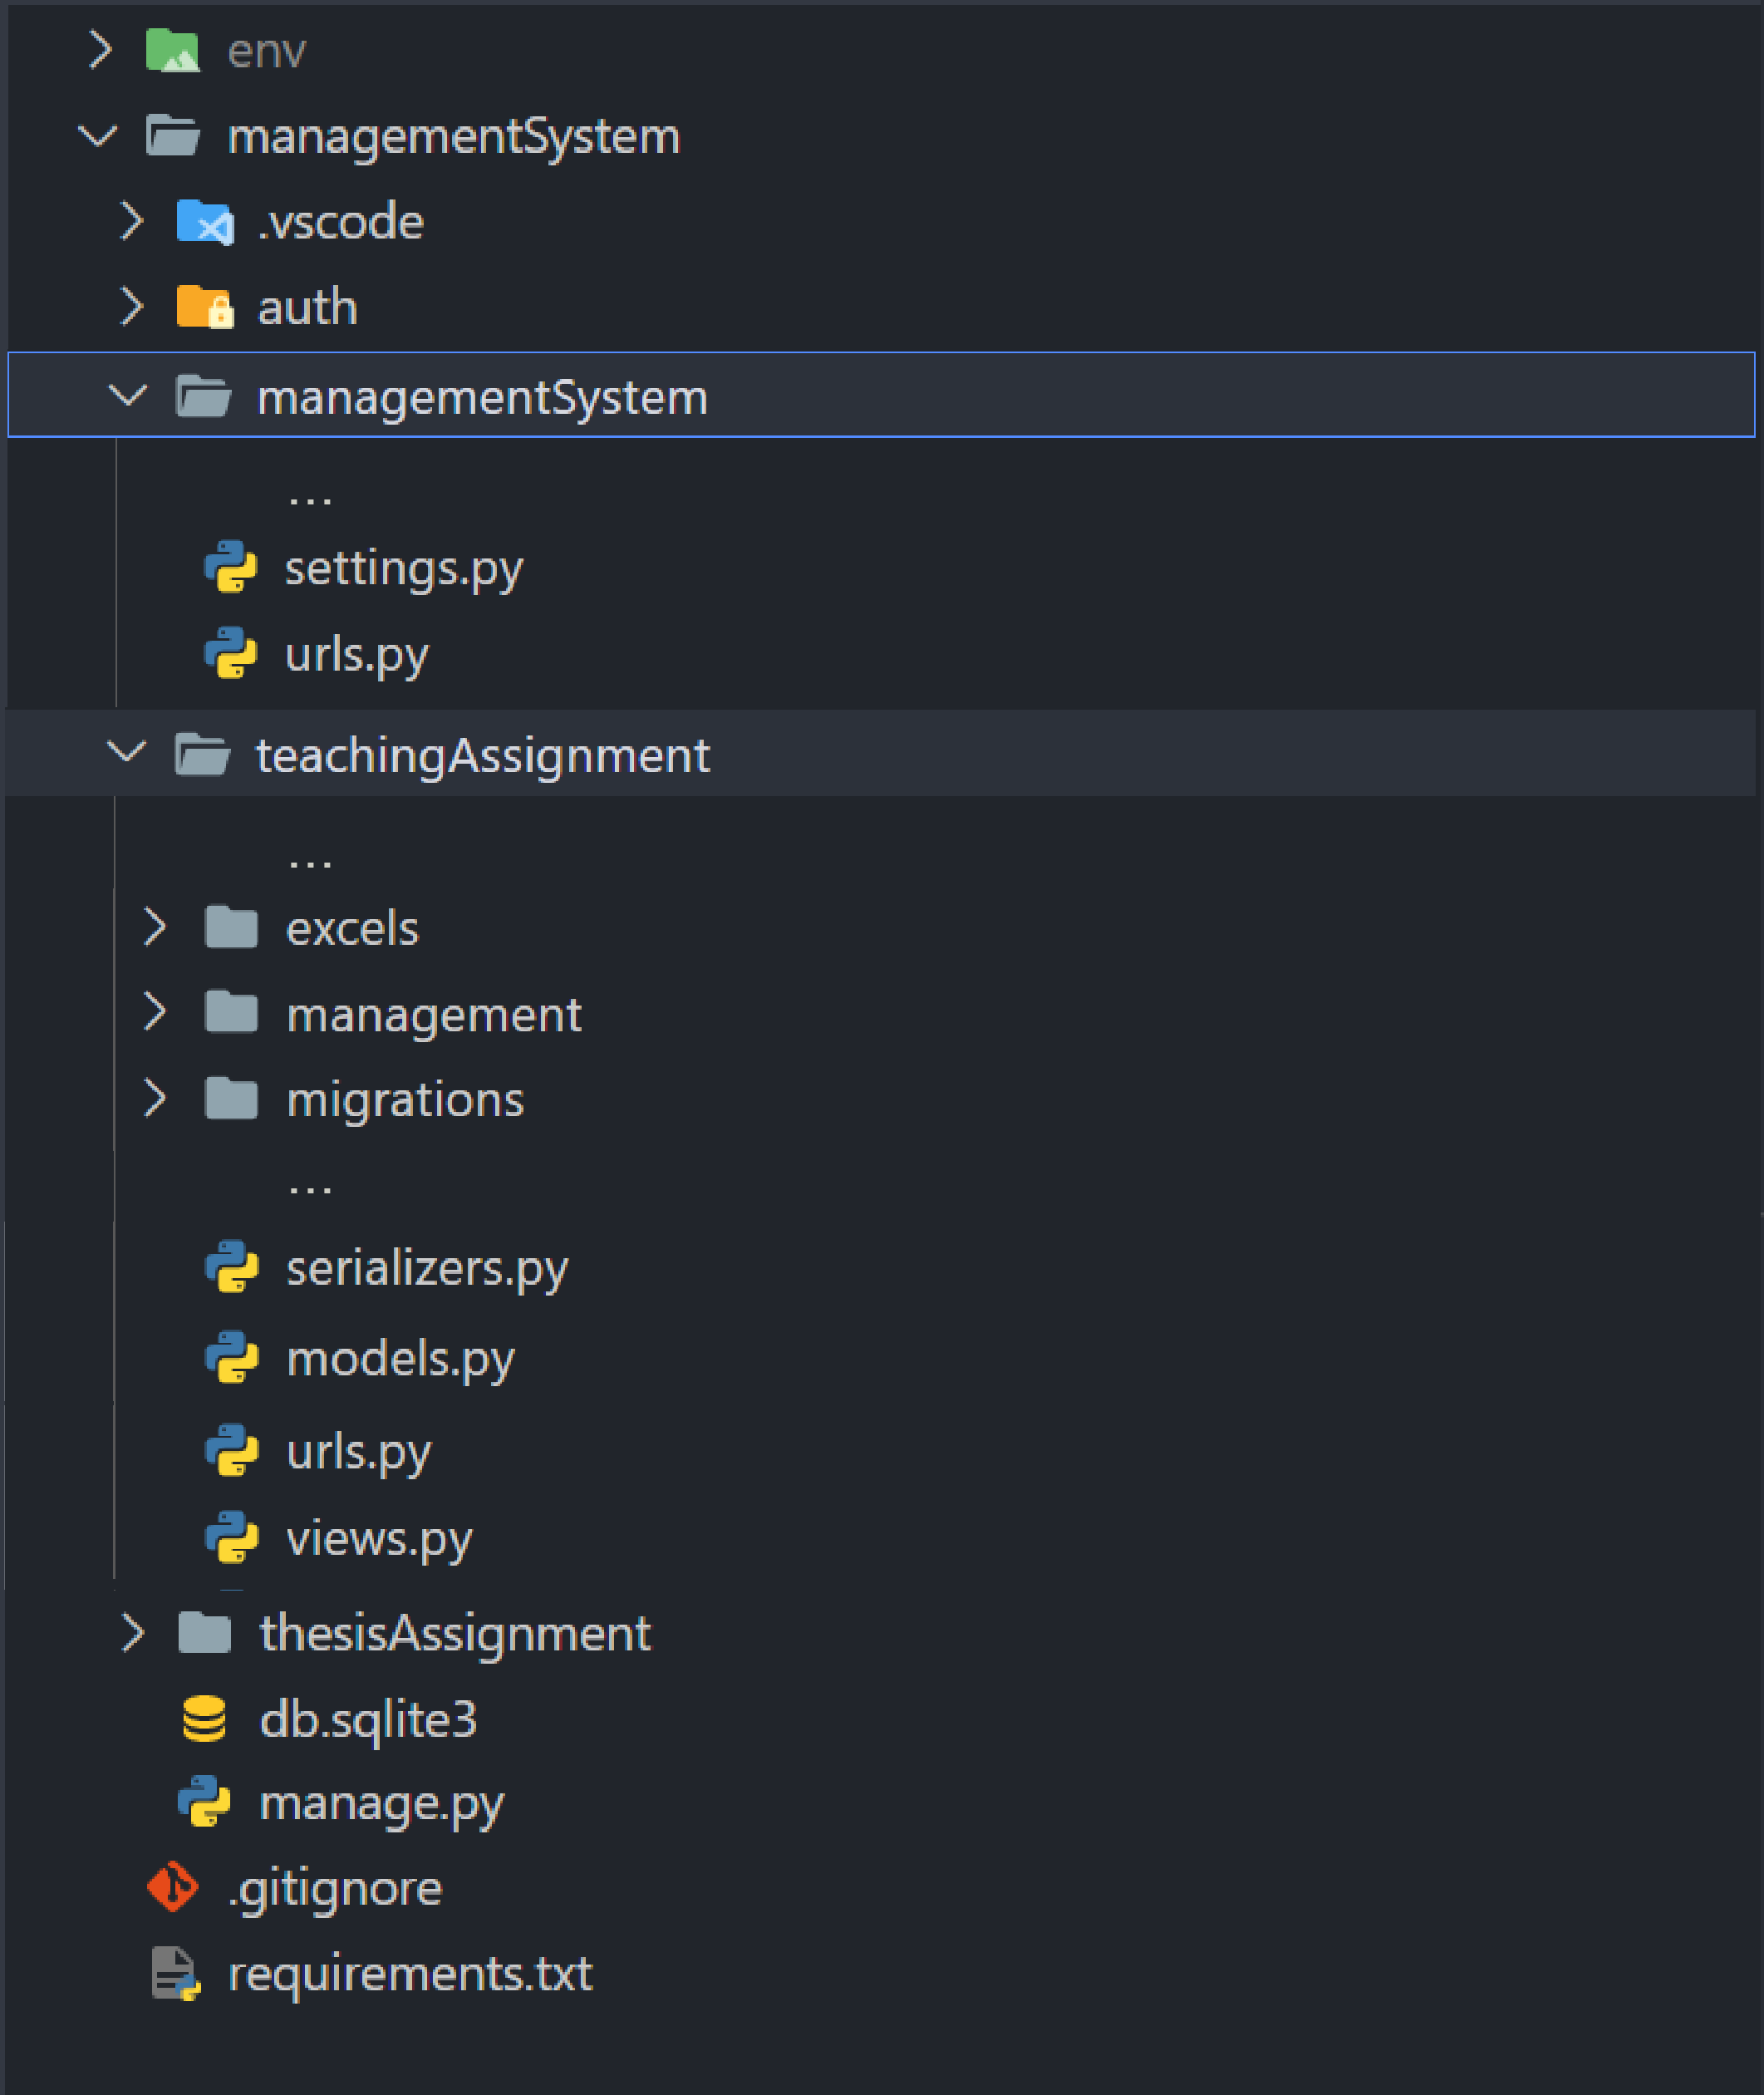
\includegraphics[scale=0.18]{Graphics/Extensibility/server-structure.png}
    \caption{Estructura de los ficheros del proyecto servidor}
    \label{img-server-structure}
\end{figure}


A continuación se describen las carpetas y ficheros principales del proyecto 
servidor.

\begin{itemize}
    \item managementSystem: es la carpeta principal del proyecto, en el fichero settings.py se encuentran
    todas las configuraciones. En el fichero url.py se deben agregar las urls de las apps creadas 
    en el proyecto. En este caso, se incluyen las urls de las apps teachingAssignment y thesisAssignment. 
    \item teachingAssignment:  app creada para el desarrollo del proceso de asignación de docencia. En la carpeta excels 
    se implementó la funcionalidad de descargar un fichero CSV con la información de la asignación de docencia. 
    \item teachingAssignment:  app creada para el desarrollo del proceso de planificación de las tesis. En la carpeta excels 
    se implementó la funcionalidad de descargar la información de los tribunales y defensas de tesis en ficheros CSV.
    \item teachingAssignment/management: en esta carpeta se encuentran las implementaciones de los comandos \textit{save\_database} 
    y \textit{fill\_database}, con los que se permite salvar y poblar la base de datos, respectivamente.
\end{itemize}


Para el desarrollo del cliente se utilizó la biblioteca Quasar. El proyecto 
cliente se inició haciendo uso de la herramienta Quasar CLI. 
La distribución de los ficheros quedó como se muestra a continuación.

\begin{figure}[H]
    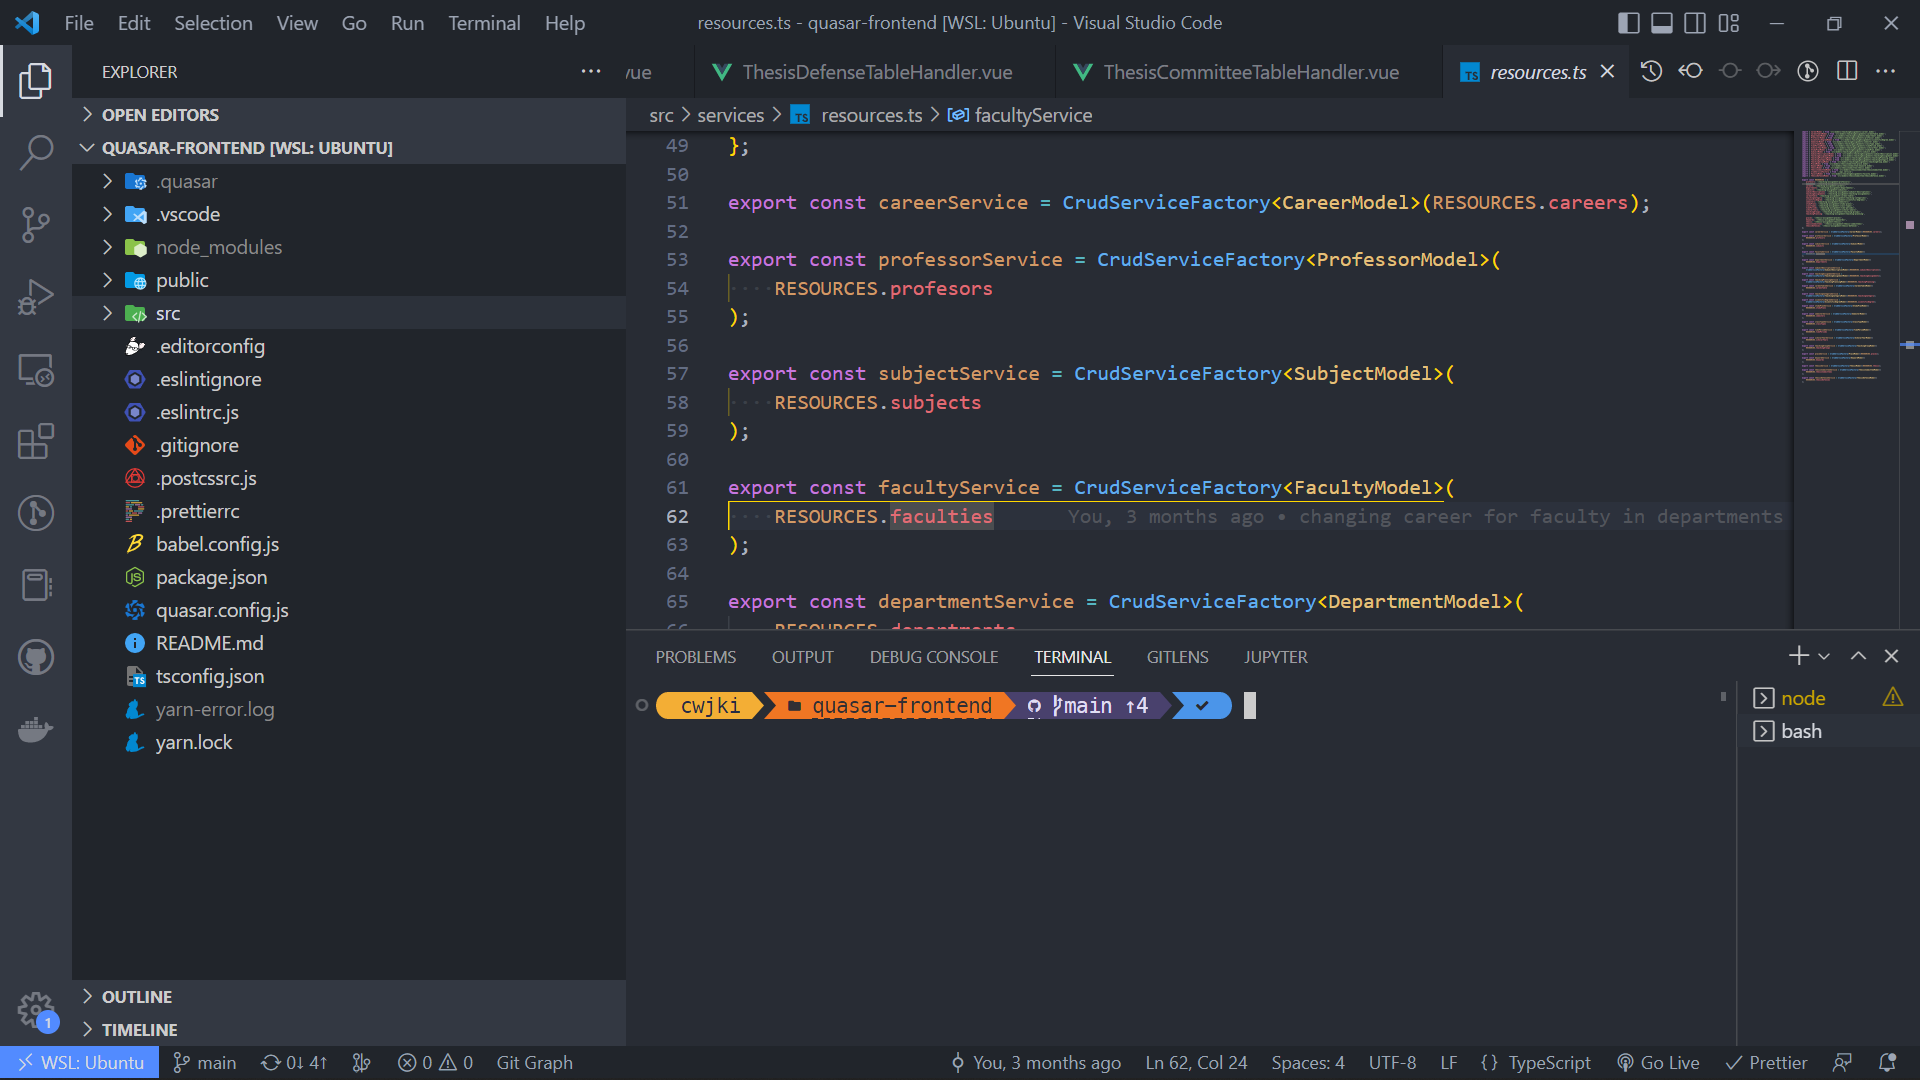
\includegraphics[scale=0.5]{Graphics/Extensibility/client-structure.png}
    \caption{Estructura de los ficheros del proyecto servidor}
    \label{img-client-structure}
\end{figure}

A continuación se describe qué encontrar en cada una de las carpetas principales del proyecto
cliente.

\begin{itemize}
    \item assets: las imágenes que se utilizaron en el proyecto.
    \item boot: se configura la url base para la comunicación con el servidor. 
    \item components: las componentes implementadas para el funcionamiento del proyecto. 
    Por ejemplo se creó una componente tabla para la visualización de cada una de las entidades 
    que intervienen en los procesos de asignación de docencia y planificación de las tesis. 
    \item css: los ficheros relacionados con el estilo utilizado.
    \item hooks: la implementación de un hook para conocer qué departamento se desea administrar en cada momento 
    y mostrar solo los datos relacionados con ese departamento. Por ejemplo, si se quiere realizar la asignación de docencia en el 
    departamento de Matemática Aplicada, solo se deben poder asignar los profesores que pertenezcan a ese departamento.
    \item layouts: la implementación del la barra de navegación principal.
    \item models: las definiciones de los tipos utilizados. Por ejemplo, se creó una interfaz ProfessorModel donde se definen los 
    campos que tiene un profesor, como: id, name, lastName, department, scientificDegree y teachingCategory.  
    \item pages: la implementación de las páginas de la aplicación web.
    \item router: el enrutamiento de la aplicación web.
    \item services: la implementación de una capa de abstracción para la comunicación con el servidor.
\end{itemize}


Se definió una capa de abstracción para la comunicación con 
el servidor, que permite a partir de una url, realizar las operaciones CRUD: create, read, update, delete. 
A continuación se muestra su definición.

\begin{verbatim}
    export const CrudServiceFactory = <T = any>(url: string) => {
    return {
        url: url,
        fullUrl: baseURL + url,
        create(obj: T) {
            return api.post<T>(url, obj);
        },
        list(query: Dictionary = {}) {
            return api.get<ListResult<T>>(url + buildQuery(query));
        },
        update(id: string, obj: Dictionary) {
            return api.patch<T>(url + id + '/', obj);
        },
        delete(id: string) {
            return api.delete<T>(url + id);
        },
    };
};
\end{verbatim}


En el fichero resources.ts, que se encuentra dentro de la carpeta ``services'',
se debe definir un servicio para cada uno de los endpoints 
con los que se quiera realizar la comunicación. Por ejemplo,
para realizar las peticiones relacionadas a los profesores se 
creó el servicio ``professorService'', cuyo definición se muestra a continuación.

\begin{verbatim}
    export const RESOURCES = {
        profesors: '/teaching-assignment/professors/',
        faculties: '/teaching-assignment/faculties/',
        careers: '/teaching-assignment/careers/',
        ...,

    };

    export const professorService = CrudServiceFactory<ProfessorModel>(
        RESOURCES.profesors
    );
\end{verbatim}


De esta forma, desde cualquier fichero que se importe el servicio ``professorService'',
se pueden realizar peticiones al servidor del estilo:

\begin{verbatim}
    professorService.create(obj: T)
    professorService.list(query: Dictionary)
    professorService.update(id: string, obj: Dictionary)
    professorService.delete(id)
\end{verbatim}


En la siguiente sección, se recomiendan las pautas a seguir para la incorporaración 
de nuevos procesos en el sistema de gestión.

\section{Recomendaciones para agregar un nuevo proceso en el sistema de gestión}
Para describir los pasos que se deben seguir para agregar un nuevo proceso en el sistema,
se ejemplificará con el proceso de planificación de las tesis. Supongamos que en el 
sistema de gestión solo está informatizado el proceso de asignación de docencia y se 
quiere agregar el de planificación de las tesis.

En el lado del servidor,
se recomienda crear una una app de django para encapsular los ficheros necesarios 
que intervienen en la modelación del proceso de planificación de las tesis.
Por tanto el primer paso sería ejecutar el siguiente comando.

\begin{verbatim}
    python manage.py startapp thesisAssignment
\end{verbatim}

Dentro de la carpeta thesisAssignment se deben definir los modelos, serializadores, 
vistas y urls necesarias. Para el proceso de planificación de las tesis se crearon nuevas 
entidades como Place, Keyword, Thesis, ThesisCommittee y ThesisDefense. Se modelaron sus
relaciones con otras entidades que se habían definido durante el proceso de asignación de 
docencia, por ejemplo, entre las entidadades Thesis y Professor se definieron las relaciones de tutor y cotutor.

En el lado del cliente, se siguieron los siguientes pasos para agregar el proceso 
de planificación de las tesis. 

\begin{itemize}
    \item Se creó la carpeta thesisCommittee, dentro de la carpeta src/models, para 
    agregar los tipos de las entidades que interviene en este proceso. Se agregaron las interfaces 
    KeywordModel, PlaceModel, ThesisModel, ThesisCommitteeModel y ThesisDefenseModel.
    \item En el fichero resources.ts, que se encuentra en la carpeta services, se crearon los servicios 
    placeService, keywordService, thesisService, thesisCommitteeService y thesisDefenseService, para realizar 
    las peticiones al servidor.
    \item Se creó una carpeta thesisCommittee dentro de la carpeta src/components/tables para agrupar 
    las componentes que se implementaron para la visualización de los datos en tablas. 
    \item Se creó una carpeta thesisCommittee dentro de la carpeta src/pages para agrupar 
    las vistas que necesarias para la modelación de este proceso: Keywords.vue, Place.vue, 
    Thesis.vue, ThesisCommittee.vue y ThesisDefense.vue.
    \item En el fichero routes.ts que se encuentra en la carpeta src/routes, se agregaron las rutas que llevan a las vistas definidas en el paso anterior.
    \item Se agregaron los botones que permiten ir a las vistas creadas en la barra de navegación de la aplicación web.
\end{itemize}


En resumen, en el lado del servidor, se recomienda la creación de una nueva app de Django que agrupe los ficheros necesarios para la modelación del 
proceso que se desea incorporar en el sistema de gestión. Se deben definir los modelos, cómo se serializan los datos y a través de cuáles urls se exponen.
En el lado del cliente se recomienda crear interfaces que representen el tipo de las entidades que intervienen en el proceso, definir los servicios para realizar 
las peticiones al servidor, agrupar las componentes y las vistas necesarias en carpetas que indiquen el proceso que se está informatizando y agregar un mecanismo para 
acceder a esas vistas. 

% Supongamos que se quiere agregar al sistema de gestión el proceso de planificación de 
% las evaluaciones de un semestre. A continuación se describen los pasos principales
% que se sugieren para la integración de este proceso.

% \begin{itemize}
%     \item Crear una nueva app de django con el comando tal.
%     \item Dentro de la carpeta creada en el paso anterior definir los modelos, serializadores, 
%     vistas y urls necesarios en ficheros nombrados models.py, serializers.py, views.py, urls.py respectivamente. 
%     \item Crear una carpeta con el nombre del proceso que se está modelando dentro de las carpetas pages y components. 
%     En la carpeta pages se encuentrar las vistar principales y dentro de la carpeta components definir las componentes 
%     necesarias 
%     \item En la carpeta services se implemetó una api para la comunicación con el servidor. Se creo un CRUDServiceFactory 
%     que permite realizar pedidos de crear, listar, actualizar y borrar. Solo se necesita agregar la url y el tipo de dato 
%     en el fichero resources. 
    

% \end{itemize}



